% This source file is part of the Geophysical Fluids Modeling Framework (GAME), which is released under the MIT license.
% Github repository: https://github.com/OpenNWP/GAME

\documentclass[10pt]{report}
\usepackage[utf8]{inputenc}
\usepackage{a4wide, amsmath, xcolor, longtable, geometry, fancyhdr, mathtools, array, listings}
\usepackage[style = numeric, backend = biber]{biblatex}
\usepackage{fouriernc}
\usepackage[T1]{fontenc}
\usepackage[hidelinks]{hyperref}
\usepackage[htt]{hyphenat}
\geometry{a4paper, top = 15mm, left = 5mm, right = 5mm, bottom = 17mm}
\fancypagestyle{plain}{
\fancyhead[L]{\texttt{GAME} handbook}
\fancyhead[R]{\textsc{\texttt{GAME} development team}}
\fancyfoot[C]{\thepage}
\addtolength\footskip{12pt}}
\definecolor{table_green}{rgb}{0, 0.6, 0}
\title{\texttt{Geophysical Fluids Modeling Framework} Handbook}
\author{\texttt{GAME} Development Team}
\date{}
\newcommand{\md}[1]{\frac{D#1}{Dt}}
\newcommand{\omegabi}{\text{{\osgbi ω}}}
\newcommand{\mubi}{\text{{\osgbi μ}}}
\newcommand{\sigmabi}{\text{{\osgbi σ}}}
\newcommand{\epsilonbi}{\text{{\osgbi ϵ}}}
\newcommand{\etabi}{\text{{\osgbi η}}}
\newcommand{\zetabi}{\text{{\osgbi ζ}}}
\addbibresource{references.bib}
\DeclareFieldFormat[article]{title}{{#1}}

\begin{document}

\maketitle

\tableofcontents

\chapter{Overview}
\label{chap:overview}

The \texttt{Geophysical Fluids Modeling Framework (GAME)} is a non-hydrostatic hexagonal C-grid dynamical core with the possibility to advect a variable number of constituents. The term \textit{dynamical core} typically refers to the simulation of a dry atmosphere, including horizontal momentum diffusion. Everything else is then referred to as \textit{physics}. Diffusive terms, including turbulence parameterizations, are sometimes understood to be part of the dynamical core and sometimes seen as part of the model's physics. The dry air is in this understanding a "carrier medium", whereas constituents, including water in different phases, are usually only passively advected. This thinking always leads to deep physical inconsistencies during later stages of model development, whose impact on forecast and climate simulation accuracy remains unknown.

Therefore, a new, capaple framework for simulating geophysical fluids is necessary and, due to the advent of even more powerful computers, also realistic. \texttt{GAME} can be seen as a dynamical core, but in a modernized sense. Its aim is to simulate the dynamics of geophysical fluid flow accurately, and at the same time make it possible to couple the model to different constituents \textit{self-consistently}, which means without violating fundamental physical constraints. For radiation, it is coupled to the \texttt{RTE+RRTMGP (Radiative Transfer for Energetics + Rapid and Accurate Radiative Transfer Model for Geophysical Circulation Model Applications—Parallel)} \cite{doi:10.1029/2019MS001621}, \cite{rte-rrtmgp-github} scheme, which follows a similar approach to radiation simulation as \texttt{GAME} follows to fluid simulation.

This is only the handbook (manual) of the \texttt{Geophysical Fluids Modeling Framework (GAME)}, it explains how to configure, compile and run (use) the model. For a scientific derivation of the model see \cite{kompendium} and the literature cited therein. The source code of the project is maintained on Github (\url{https://github.com/OpenNWP/GAME}).

The \texttt{GAME} project incorporates two different executables:

\begin{itemize}
\item \texttt{grid\_generator}, a program for creating model grids
\item \texttt{game}, the model executable itself
\end{itemize}

\chapter{Code structure}
\label{chap:code_structure}

The code of the model resides in the directory \texttt{src}.

\section{Spatial operators}
\label{sec:spatial_operators}

\begin{itemize}
\item Coriolis: \cite{thuburn_f_discrete_plane} and \cite{ringler_trsk} modified by \cite{doi:10.1002/qj.3294}
\item kinetic energy: \cite{ringler_trsk}
\end{itemize}

\section{Time stepping}
\label{sec:time_stepping}

A fully Eulerian time stepping is employed. The basic building structure is a two-time-level predictor-corrector scheme. In the vertical, at every substep, an implicit column solver is used, which makes it possible to violate the CFL criterion of vertically propagating sound and fast gravity waves. This has the cost of decreasing the accuracy of these modes, which is however a bearable trade-off, since these waves are of low meteorological relevance. Furthermore, a forward-backward scheme is used, where the divergence term is backward.

\chapter{Installation}
\label{chap:installation}

It is recommended to run the model on Linux. These installation instructions are tested for Ubuntu, for other Linux distributions they might have to be modified.

\section{Dependencies}
\label{sec:dependencies}

The following dependencies must be installed before being able to successfully build the model:

\begin{itemize}
\item \texttt{sudo apt-get install gfortran make cmake wget python3-pip libnetcdff-dev}
\item Clone the RTE+RRTMGP repository: \texttt{git clone https://github.com/earth-system-radiation/rte-rrtmgp}
\item The Python visualization library scitools-iris (installation manual: \url{https://scitools-iris.readthedocs.io/en/stable/installing.html#installing-from-source-without-conda-on-debian-based-linux-distros-developers}, only for the plotting routines)
\item FFMPEG (\texttt{sudo apt-get install ffmpeg}, only for the plotting routines)
\end{itemize}

\section{Building}
\label{sec:building}

\texttt{CMake} is used for building \texttt{GAME}. Execute \texttt{./compile.sh} to build the model. The following flags can be used with \texttt{./compile.sh}:
%
\begin{itemize}
\item \texttt{-d}: debugging flags (\texttt{-fbounds-check -Wall -Wno-c-binding-type -ffpe-trap=invalid,zero,overflow -fbacktrace -fdump-core})
\item \texttt{-f}: more aggressive optimization (\texttt{O3} instead of \texttt{O2})
\item \texttt{-c}: compile-time configuration of the model for more performance
\item \texttt{-s}: single precision
\end{itemize}

\chapter{Grid generation}
\label{chap:grid_generation}

\begin{figure}
\begin{center}
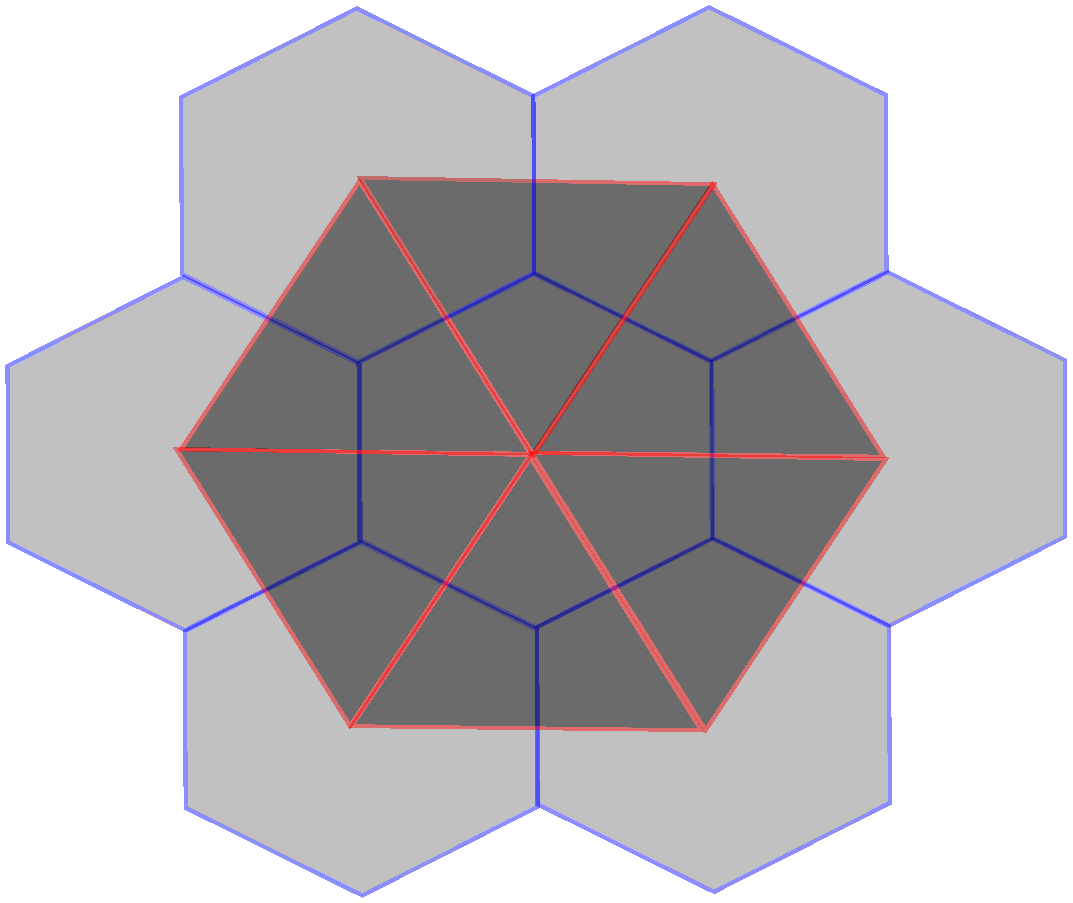
\includegraphics[width = 0.6\textwidth]{hexagonal_grid_0.pdf}
\caption{A subset of a regular horizontal hexagonal grid. The hexagonal grid (blue lines) and the triangular grid (red lines) form a pair of a primal-dual grid. In \texttt{GAME}, the hexagonal grid is the primal grid, while the triangulars form the dual one. In a triangular grid model it is the other way around. During the grid generation procedure we refer to the triangle edge points (hexagon centers) as the generating points or generators, for short.}
\label{fig:hexagonal_grid_0}
\end{center}
\end{figure}

\section{Fundamental grid quantities}
\label{sec:fundamental_grid_quantities}

The following quantities are sufficient to uniquely define the grid:

\begin{itemize}
\item the horizontal coordinates of the generating points
\item the numbering of the generating points
\item the numbering and orientation of the horizontal vectors
\item the numbering of the dual cell mid points
\item The orientation of the dual horizontal vectors. Since their horizontal positions coincide with the horizontal positions of the primal vectors, both sets of vectors can be numbered in the same way.
\end{itemize}
%
All other quantities, be it floating point numbers like grid box volumes or areas, or integer quantities like neighborhood relationships, can be implicitly derived. Consequently, once must firstly focus on the fundamental grid properties.

\subsection{Creating a spherical geodesic grid}
\label{sec:creating_a_spherical_geodesic_grid}

By \textit{horizontal grid} we mean the grid on one single layer. Without loss of generality this layer can be assumed to coincide with the surface of the unit sphere.

\subsection{Numbering and orienting the vector points}
\label{sec:numbering_and_orienting_the_vector_points}

\subsection{Numbering and orienting the dual vector points}
\label{sec:numbering_and_orienting_the_dual_vector_points}

Until now, we have only operated with the six following arrays:
%
\begin{itemize}
\item \texttt{latitude\_scalar}, \texttt{longitude\_scalar}
\item \texttt{from\_index}, \texttt{to\_index}
\item \texttt{from\_index\_dual}, \texttt{to\_index\_dual}
\end{itemize}
%

\section{Derived quantities}
\label{sec:derived_quantities}

\subsection{Horizontal coordinates of dual scalar points}
\label{sec:horizontal_coordinates_of_dual_scalar_points}

The dual cells of a hexagonal grid are the triangular grid cells. Since we aim at an orthogonal grid, the dual scalar points must be the Voronoi centers of the triangular cells. Label the vertices of one triangle with $\mathbf{r}_0, \mathbf{r}_1, \mathbf{r}_2$, then its Voronoi center $\mathbf{r}_v$ is located at the position
%
\begin{align}
\mathbf{r}_v \coloneqq \frac{\left(\mathbf{r}_1 - \mathbf{r}_0\right)\times\left(\mathbf{r}_2 - \mathbf{r}_0\right)}{\left|\left(\mathbf{r}_1 - \mathbf{r}_0\right)\times\left(\mathbf{r}_2 - \mathbf{r}_0\right)\right|}.
\end{align}

\subsection{Finding the neighboring vector points of a primal cell and their orientation}
\label{sec:finding_the_neighboring_vector_points_of_a_primal_cell_and_their_orientation}

\begin{figure}
\begin{center}
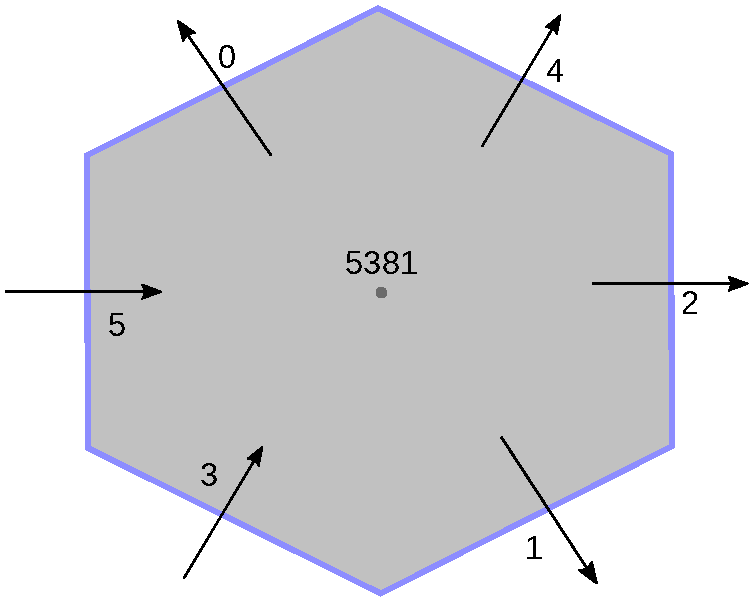
\includegraphics[width = 0.5\textwidth]{hexagonal_grid_1.pdf}
\caption{A sample hexagon with a horizontal scalar index of 5381. The directions of the arrows indicate the directions of unit vectors at cell edges. The drawn orientations would lead to $\texttt{adjacent\_vector\_signs\_h}(1,5381) = 1$, $\texttt{adjacent\_vector\_signs\_h}(2,5381) = 1$, $\texttt{adjacent\_vector\_signs\_h}(3,5381) = -1$, $\texttt{adjacent\_vector\_signs\_h}(4,5381) = 1$, $\texttt{adjacent\_vector\_signs\_h}(5,5381) = -1$, $\texttt{adjacent\_vector\_signs\_h}(6,5381) = 1$.}
\label{fig:hexagonal_grid_1}
\end{center}
\end{figure}

\subsection{Finding the neighboring vector points of a dual cell and their orientation}
\label{sec:finding_the_neighboring_vector_points_of_a_dual_cell_and_their_orientation}

\section{Grid optimization}
\label{sec:grid_optimization}

Hexagonal spherical grids need to be optimized for numerical modeling. Therefore, the Lloyd algorithm is used, which yields a \textit{spherical centroidal Voronoi tesselation (SCVT)} after convergence \cite{Du2003}. \cite{PEIXOTO201361} gives an overview of optimization alternatives and it seems to be that the SCVT is the most suitable for modeling. The procedure employed for executing the Lloyd algorithm is the one described in \cite{10.1175/MWR2991.1}.

\section{Vertical grid structure}
\label{sec:vertical_grid_structure}

So far, only a horizontal grid has been examined. The grid generator, however, shall produce full three-dimensional grids. In order to simplify matters, the following conventions are made:
%
\begin{itemize}
\item Since the vertically oriented primal vector points have the same horizontal coordinates as the primal scalar points, their horizontal numbering is also the same.
\item Since the vertically oriented dual vector points have the same horizontal coordinates as the dual scalar points, their horizontal numbering is also the same.
\end{itemize}

\section{Scalability}
\label{sec:scalability}

The computation time of the most expensive for loops scale with $N^2$, where $N$ is the number of horizontal grid points. This means that doubling the horizontal resolution (four times as much horizontal grid points) leads to a 16 times longer computation time of the grid generator. This is similar to the model itself, where a doubling of the horizontal and vertical resolution and a halfening of the time step leads to 16 times longer integration times. Therefore, the largely implicit formulation of the grid generator poses no problem to its performance at higher resoultions.

\subsection{Permutations of the grid points}
\label{sec:permutations_of_the_grid_points}

\section{Horizontal grid properties}
\label{sec:horizontal_grid_properties}

The horizontal grid structure is determined by the following properties:

\begin{itemize}
\item the resolution, specified via the parameter \texttt{RES\_ID}
\item the optimization
\end{itemize}

\section{Vertical grid properties}
\label{sec:vertical_grid_properties}

The vertical grid structure is determined by the following properties:

\begin{itemize}
\item the height of the top of the atmosphere, specified via the parameter \texttt{TOA}
\item the number of layers, specified via the parameter \texttt{NO\_OF\_LAYERS} $N_L$
\item the number of layers following the orography, specified via the parameter \texttt{NO\_OF\_ORO\_LAYERS} $N_O$
\item the stretching parameter $\beta$, which can be set in the run script
\item the orography, specified via the parameter \texttt{oro\_id}
\end{itemize}

The generation of the vertical position of the grid points works in three steps:
%
\begin{enumerate}
\item First of all, vertical positions of preliminary levels with index $0 \leq j \leq N_L$ are determined by
%
\begin{align}
z_j = T\sigma_{z, j} + B_jz_S,
\end{align}
%
where $T$ is the top of the atmosphere, $\sigma_{z, j}$ is defined by
%
\begin{align}
\sigma_{z, j} \coloneqq \left(1 - \frac{j}{N_L}\right)^\alpha,
\end{align}
%
where $\alpha \geq 1$ is the so-called \textit{stretching parameter}, $z_s$ is the surface height and $B_j$ is defined by
%
\begin{align}
B_j \coloneqq \frac{j - \left(N_L - N_O\right)}{N_O}.
\end{align}
%
\item Then, the scalar points are positioned in the middle between the adjacent preliminary levels.
\item Then, the vertical vector points are regenerated by placing them in the middle between the two adjacent layers.
\item Finally, the vertical positions of the other points are diagnozed through interpolation.
\end{enumerate}

\section{How to generate a grid}
\label{sec:how_to_generate_a_grid}

Use the bash script \texttt{grid\_generator/compile.sh} to compile the grid generator. Then run the grid generator using the bash script \texttt{grid\_generator/run\_script.sh} with the desired \texttt{\texttt{oro\_id}}. Table \ref{tab:grid_generator_run_file_explanation} explains all the parameters to be set in \texttt{grid\_generator/run\_script.sh}.

\renewcommand{\arraystretch}{1.2}
\begin{table}
\centering
\begin{tabular}{|>{\centering}p{5.0 cm}|>{\centering}p{3 cm}|>{\centering}p{7 cm}|}
\hline \textbf{name} & \textbf{domain} & \textbf{meaning} \tabularnewline
\hline\hline \texttt{\texttt{res\_id}} & $\geq 4$ & resolution ID \tabularnewline
\hline\hline \texttt{\texttt{oro\_id}} & 0,1 & orography ID \tabularnewline
\hline\hline \texttt{n\_lloyd\_iterations} & integer $\geq$ 0 & number of iterations of the Lloyd algorithm, 2000 is a reasonable value \tabularnewline
\hline\hline \texttt{luse\_scalar\_h\_file} & boolean & switch to determine wether fundamental horizontal grid properties shall be read from a previously generated file \tabularnewline
\hline\hline \texttt{luse\_sfc\_file} & boolean & switch to determine wether physical surface properties shall be read from a file \tabularnewline
\hline\hline \texttt{scalar\_h\_coords\_file} & string & input file for dual triangle vertices (only relevant if \texttt{use\_scalar\_h\_coords\_file} = 1) \tabularnewline
\hline\hline \texttt{stretching\_parameter} & $\geq 1$, real & defines the vertical stretching of the grid, one means no stretching \tabularnewline
\hline\hline \texttt{toa} & $> 0$, real & height of the top of the atmosphere \tabularnewline
\hline\hline \texttt{n\_oro\_layers} & $\geq$ 1, natural & number of layers following orography (only relevant if \texttt{type\_of\_vertical\_grid} == 0) \tabularnewline
\hline\hline \texttt{radius\_rescale} & $> 0$, real & rescale factor for the radius of the grid, radius $r$ will be calculated according to $r = \texttt{radius\_rescale}\cdot a$, where $a$ is the Earth radius; angular velocity $\omega$ will be replaced according to $\omega \to \frac{\omega}{\texttt{radius\_rescale}}$ \tabularnewline
\hline\hline \texttt{n\_avg\_points} & $\geq$ 1 & number of points used for smoothing the orography \tabularnewline
\hline\hline \texttt{lsleve} & boolean & switch for the SLEVE vertical coordinate smoothing technique \tabularnewline
\hline
\end{tabular}
\caption{Grid generator run script explanation.}
\label{tab:grid_generator_run_file_explanation}
\end{table}
\renewcommand{\arraystretch}{1}

\section{Physical surface properties}
\label{sec:physical_surface_properties}

The properties of the surface of the Earth influence the evolution of the atmospheric fields. Therefore, physical surface properties need to be obtained from external sources and interpolated to the model grid. The following fields are required:
%
\begin{itemize}
\item The land distribution. source: \url{https://ral.ucar.edu/sites/default/files/public/product-tool/noah-multiparameterization-land-surface-model-noah-mp-lsm/usgs/sfc-fields-usgs-veg30susgs.gz} \cite{glcc}
\item The orography. source: \url{https://www.ngdc.noaa.gov/mgg/global/relief/ETOPO1/data/ice_surface/grid_registered/netcdf/ETOPO1_Ice_g_gmt4.grd.gz} \cite{etopo1}, \cite{etopo1_add}
\item The lake fraction (share of a grid cell covered by lakes). source: \url{http://www.flake.igb-berlin.de/data/gldbv2.tar.gz} \cite{gldb}
\item The global mean of the 2-m-temperature as the lower boundary condition of the soil temperature. source: \url{https://downloads.psl.noaa.gov/Datasets/ghcncams/Derived/air.mon.ltm.nc} \cite{GHCN_CAMS}
\item The density of the soil.
\item The specific heat capacity of the soil.
\item The temperature diffusivity of the soil.
\item For NWP runs without coupling to an ocean model, the SST needs to be prescribed in order to calculate sensible and latent heating rates at the ocean surface (actually, we use the near sea surface temperature (NSST)). source: \url{https://nomads.ncep.noaa.gov/pub/data/nccf/com/nsst/prod/} (The SST is set analytically for idealized simulations.)
\item The land-sea mask of the NCEP NSST data. source: \url{https://downloads.psl.noaa.gov/Datasets/noaa.oisst.v2/lsmask.nc}
\end{itemize}

\renewcommand{\arraystretch}{1.2}
\begin{table}
\centering
\begin{tabular}{|>{\centering}p{4.0 cm}|>{\centering}p{8 cm}|}
\hline \textbf{\texttt{oro\_id}} & \textbf{Description} \tabularnewline
\hline\hline 0 & no orography \tabularnewline
\hline 1 & real orography \tabularnewline
\hline
\end{tabular}
\caption{Definition of orography IDs.}
\label{tab:oro_id_definition}
\end{table}
\renewcommand{\arraystretch}{1}

Tab. \ref{tab:oro_id_definition} shows the definition of the orography IDs. Before creating a grid file with real orography (orography ID 1), you have to create a grid file of orography ID 0.

\chapter{Ideal test states}
\label{chap:ideal_test_states}

\renewcommand{\arraystretch}{1.2}
\begin{table}
\centering
\begin{tabular}{|>{\centering}p{4.0 cm}|>{\centering}p{8 cm}|}
\hline \textbf{\texttt{TEST\_ID}} & \textbf{Description} \tabularnewline
\hline\hline 0 & standard atmosphere \tabularnewline
\hline 1 & dry Ullrich test \tabularnewline
\hline 2 & moist Ullrich test \tabularnewline
\hline
\end{tabular}
\caption{Definition of test IDs.}
\label{tab:test_id_definition}
\end{table}
\renewcommand{\arraystretch}{1}

\chapter{Running the model}
\label{chap:running_the_model}

The model is configured via the namelist residing in the directory \texttt{src/namelists}. The default parameters can be modified in the run scripts, which are the files contained in the directory \texttt{run\_scripts}.

\section{Dynamics configuration}
\label{sec:dynamics_configuration}

\section{Physics configuration}
\label{sec:physics_configuration}

\section{Coupling to the radiation field}
\label{sec:coupling_to_the_radiation_field}

\texttt{GAME} employs the so-called \texttt{RTE+RRTMGP (Radiative Transfer for Energetics + Rapid and Accurate Radiative Transfer Model for Geophysical Circulation Model Applications—Parallel)} \cite{doi:10.1029/2019MS001621}, \cite{rte-rrtmgp-github} scheme.

\section{Configuring output}
\label{sec:configuring_output}

\subsection{Output on pressure levels}
\label{sec:output_on_pressure_levels}

In meteorology, atmospheric fields are often visualized on pressure levels. To simply this, \texttt{GAME} can interpolate data to pressure levels. This can be turned on and off with the variable \texttt{pressure\_level\_output\_switch} in the run scripts.

\appendix

\printbibliography

\end{document}













